%%%%%%%%%%%%%%%%%%%%%%%%%%%%%%%%%%%%%%%%%
% baposter Landscape Poster
% LaTeX Template
% Version 1.0 (11/06/13)
%
% baposter Class Created by:
% Brian Amberg (baposter@brian-amberg.de)
%
% This template has been downloaded from:
% http://www.LaTeXTemplates.com and modified by Antonius Torode
%
% License:
% CC BY-NC-SA 3.0 (http://creativecommons.org/licenses/by-nc-sa/3.0/)
%
%%%%%%%%%%%%%%%%%%%%%%%%%%%%%%%%%%%%%%%%%

%----------------------------------------------------------------------------------------
%	PACKAGES AND OTHER DOCUMENT CONFIGURATIONS
%----------------------------------------------------------------------------------------

\documentclass[landscape,a0paper,fontscale=0.285]{baposter} % Adjust the font scale/size here

\usepackage{graphicx} % Required for including images
\graphicspath{{figures/}} % Directory in which figures are stored

\usepackage{amsmath} % For typesetting math
\usepackage{amssymb} % Adds new symbols to be used in math mode

\usepackage{booktabs} % Top and bottom rules for tables
\usepackage{enumitem} % Used to reduce itemize/enumerate spacing
\usepackage{palatino} % Use the Palatino font
\usepackage[font=small,labelfont=bf]{caption} % Required for specifying captions to tables and figures

\usepackage{multicol} % Required for multiple columns
\setlength{\columnsep}{1.5em} % Slightly increase the space between columns
\setlength{\columnseprule}{0mm} % No horizontal rule between columns

\usepackage{tikz} % Required for flow chart
\usetikzlibrary{shapes,arrows} % Tikz libraries required for the flow chart in the template

\newcommand{\compresslist}{ % Define a command to reduce spacing within itemize/enumerate environments, this is used right after \begin{itemize} or \begin{enumerate}
\setlength{\itemsep}{1pt}
\setlength{\parskip}{0pt}
\setlength{\parsep}{0pt}
}

\definecolor{lightblue}{rgb}{0.145,0.6666,1} % Defines the color used for content box headers


\begin{document}
	
\background{%
	\begin{tikzpicture}
	[remember picture,overlay]\node[opacity=1] at (current page.center) {
\includegraphics[width=\paperwidth,height=\paperheight]{BG3.jpg}};
	\end{tikzpicture}%
}

\begin{poster}
{
headerborder=closed, % Adds a border around the header of content boxes
colspacing=1em, % Column spacing
background=user,
%bgColorOne=white, % Background color for the gradient on the left side of the poster
%bgColorTwo=white, % Background color for the gradient on the right side of the poster
borderColor=lightblue, % Border color
headerColorOne=black, % Background color for the header in the content boxes (left side)
headerColorTwo=lightblue, % Background color for the header in the content boxes (right side)
headerFontColor=white, % Text color for the header text in the content boxes
boxColorOne=white, % Background color of the content boxes
textborder=roundedleft, % Format of the border around content boxes, can be: none, bars, coils, triangles, rectangle, rounded, roundedsmall, roundedright or faded
eyecatcher=true, % Set to false for ignoring the left logo in the title and move the title left
headerheight=0.1\textheight, % Height of the header
headershape=roundedright, % Specify the rounded corner in the content box headers, can be: rectangle, small-rounded, roundedright, roundedleft or rounded
headerfont=\Large\bf\textsc, % Large, bold and sans serif font in the headers of content boxes
%textfont={\setlength{\parindent}{1.5em}}, % Uncomment for paragraph indentation
linewidth=2pt % Width of the border lines around content boxes
}
%----------------------------------------------------------------------------------------
%	TITLE SECTION 
%----------------------------------------------------------------------------------------
%
{
\includegraphics[height=4em]{MSU.jpg}} % First university/lab logo on the left
{\bf\textsc{Zeeman Effect}\vspace{0.5em}} % Poster title
{\textsc{Antonius Torode and Eric Aboud -  \hspace{12pt} Michigan State University \\ Department of Physics \& Astronomy}} % Author names and institution
{
\includegraphics[height=4em]{MSU.jpg}} % Second university/lab logo on the right

%----------------------------------------------------------------------------------------
%	OBJECTIVES
%----------------------------------------------------------------------------------------

\headerbox{Introduction \& History}{name=objectives,column=0,row=0}{

Named after the Dutch physicist Hendrik Casimir, the Casimir effect is a physical force that arises from and is explained by quantized fields in quantum field theory. The typical example of this is an apparent attraction created between two very closely placed parallel plates within a vacuum. Due to the nature of quantized fields dealing with virtual particles in a vacuum, a force becomes present in the system.

\vspace{0.3em} % When there are two boxes, some whitespace may need to be added if the one on the right has more content
}

%----------------------------------------------------------------------------------------
%	Discovery & Properties
%----------------------------------------------------------------------------------------

\headerbox{Discovery \& Properties }{name=introduction,column=3,row=0,bottomaligned=objectives}{

All bosons make a contribution to the Casimir force, but fermions make a repulsive contribution to the force. Even though all of these particles make a contribution to the force, only that from photons is measurable. The theory states that the lowest energy state of a vacuum is infinite when considering all possible photon modes. The Casimir force comes about from a situation in which the differences in infinities cancel out.
}

%----------------------------------------------------------------------------------------
%	Derivation of the Casimir Force
%----------------------------------------------------------------------------------------

\headerbox{Derivation of Induced Electric Field}{name=results,column=1,span=2,row=0}{

\begin{multicols}{2}
Let $k_x$ and $k_y$ represent the wave numbers in the $x$ and $y$ directions respectively and $k_n=n\pi/a$. If we allow two plates to be parallel in the $x-y$ plane at a distance $a$ apart, the standing waves are
\begin{align}
\psi_n(x,y,z;t)= e^{ik_xx+ik_yy-i\omega_nt}\sin(k_nz).
\end{align}
The frequency of this wave is $\omega_n = c \sqrt{k_x^2+k_y^2+k_n^2}$. The vacuum energy is the sum over all possible expectation modes. Taking the expectation value of the energy yields
\begin{align}
\langle E \rangle = \frac{A\hbar}{4\pi^2} \iint \sum_{n=1}^{\infty}\omega_ndk_xdk_y.
\end{align}
This expression is clearly infinite due to the diverging sum. If we use zeta-regulation, we can find a finite energy per unit area which is
\begin{align}
\frac{\langle E(s) \rangle}{A} = \frac{\hbar}{4\pi^2} \iint \sum_{n=1}^{\infty}\omega_n|\omega|^{-s}dk_xdk_y.
\end{align}
Simplifying the above expression gives us
\begin{align}
\frac{\langle E(s) \rangle}{A} = \frac{\hbar c^{1-s}\pi^{2-s}}{{2a^{3-s}(3-s)}}\sum_{n=1}^{\infty}|n|^{3-s}.
\end{align}
This expression may be analytically continued to $s=0$ where it becomes finite. 
\begin{align}
\frac{\langle E \rangle}{A} = \lim_{s\rightarrow 0}\frac{\langle E(s) \rangle}{A} = -\frac{\hbar c \pi^2}{6a^3}\zeta(-3).
\end{align}
Now, plugging in (\ref{eq:ZetaNeg3}) to the above expression gives us
\begin{align}
\frac{\langle E \rangle}{A} = \frac{-\hbar c \pi^2}{720a^3}.
\end{align}
The Casimir force per unit area between two parallel plates within a vacuum is therefore given by $F=-\nabla \langle E \rangle$ which is
\begin{align}
\frac{F_c}{A} = -\frac{d}{da}\frac{\langle E \rangle}{A} = \frac{-\hbar c \pi^2}{240a^4}.
\end{align}
\hspace{1cm} %just fixes up the spacing by adding a blank line.
\end{multicols}
}

%----------------------------------------------------------------------------------------
%	REFERENCES
%----------------------------------------------------------------------------------------

\headerbox{References}{name=references,column=0,above=bottom}{


\scriptsize{ % Reduce the font size in this block
\begin{enumerate}
\itemsep0em 
\item John Baez on the number 24. The Rankin Lectures 2008. Youtube. John Baez. University of California. 16 May. 2012. Web. \label{baez}
\item Gibbs, Philip. "What Is the Casimir Effect?" The Casimir Effect. University of California, 1997. Web. 16 Oct. 2016. 
\item Ramanujan Aiyangar, Srinivasa, 1887-l  920. Ramanujans notebooks. Mathematics-Collected works. 1. Berndt, Bruce C., 1939- II. Title. QA3. R33. 1985. 510. 84-20201 \label{ramanujin}

\end{enumerate}
}}

%----------------------------------------------------------------------------------------
%	Addendum and Final Remarks
%----------------------------------------------------------------------------------------

\headerbox{Addendum and Final Remarks }{name=futureresearch,column=1,span=2,aligned=references,above=bottom}{ % This block is as tall as the references block
\begin{multicols}{2}
As we can clearly see, the Casimir force would not have come about without the use of analytical continuation. In a sense, this is due to nature not containing apparent infinities. Rather, the continuation allowed us to arrive at a finite solution which is experimentally confirmed. The facet that our expression came out negative suggests that the force is an attractive force, and due to the presence of $\hbar$, we can see that the force is of a quantum origin. In the original derivation, Casimir computed non-convergent sums using Euler-Maclaurin summation with a regularizing function [\ref{casimir}]
\end{multicols}
}

%----------------------------------------------------------------------------------------
%	References RIGHT
%----------------------------------------------------------------------------------------

\headerbox{References}{name=contact,column=3,aligned=references,above=bottom}{ % This block is as tall as the references block

\scriptsize{ % Reduce the font size in this block
	\begin{enumerate}
		\setcounter{enumi}{3}
		\itemsep0em 
		\item Casimir Effect \& Black Holes - Sixty Symbols. Prod. Brady Haran. Perf. Mike Merrifield Ph.D. Youtube. University of Nottingham, 20 Mar. 2014. Web. 
		\item H.B.G. Casimir, Proc. Kon. Ned. Akad. Wetensch. B51, 793 (1948) \label{casimir}
		\item Sum of Natural Numbers (second proof and extra footage). Prod. Brady Haran. Perf. Ed Copeland Ph.D and Tony Padilla Ph.D. Youtube. University of Nottingham, 11 Jan. 2015. Wb.
	\end{enumerate}
}}

%----------------------------------------------------------------------------------------
%	Implications and Applications
%----------------------------------------------------------------------------------------

\headerbox{Implications and Applications}{name=conclusion,column=1,span=2,row=0,below=results,above=references}{

\begin{multicols}{2}
	\begin{center}
		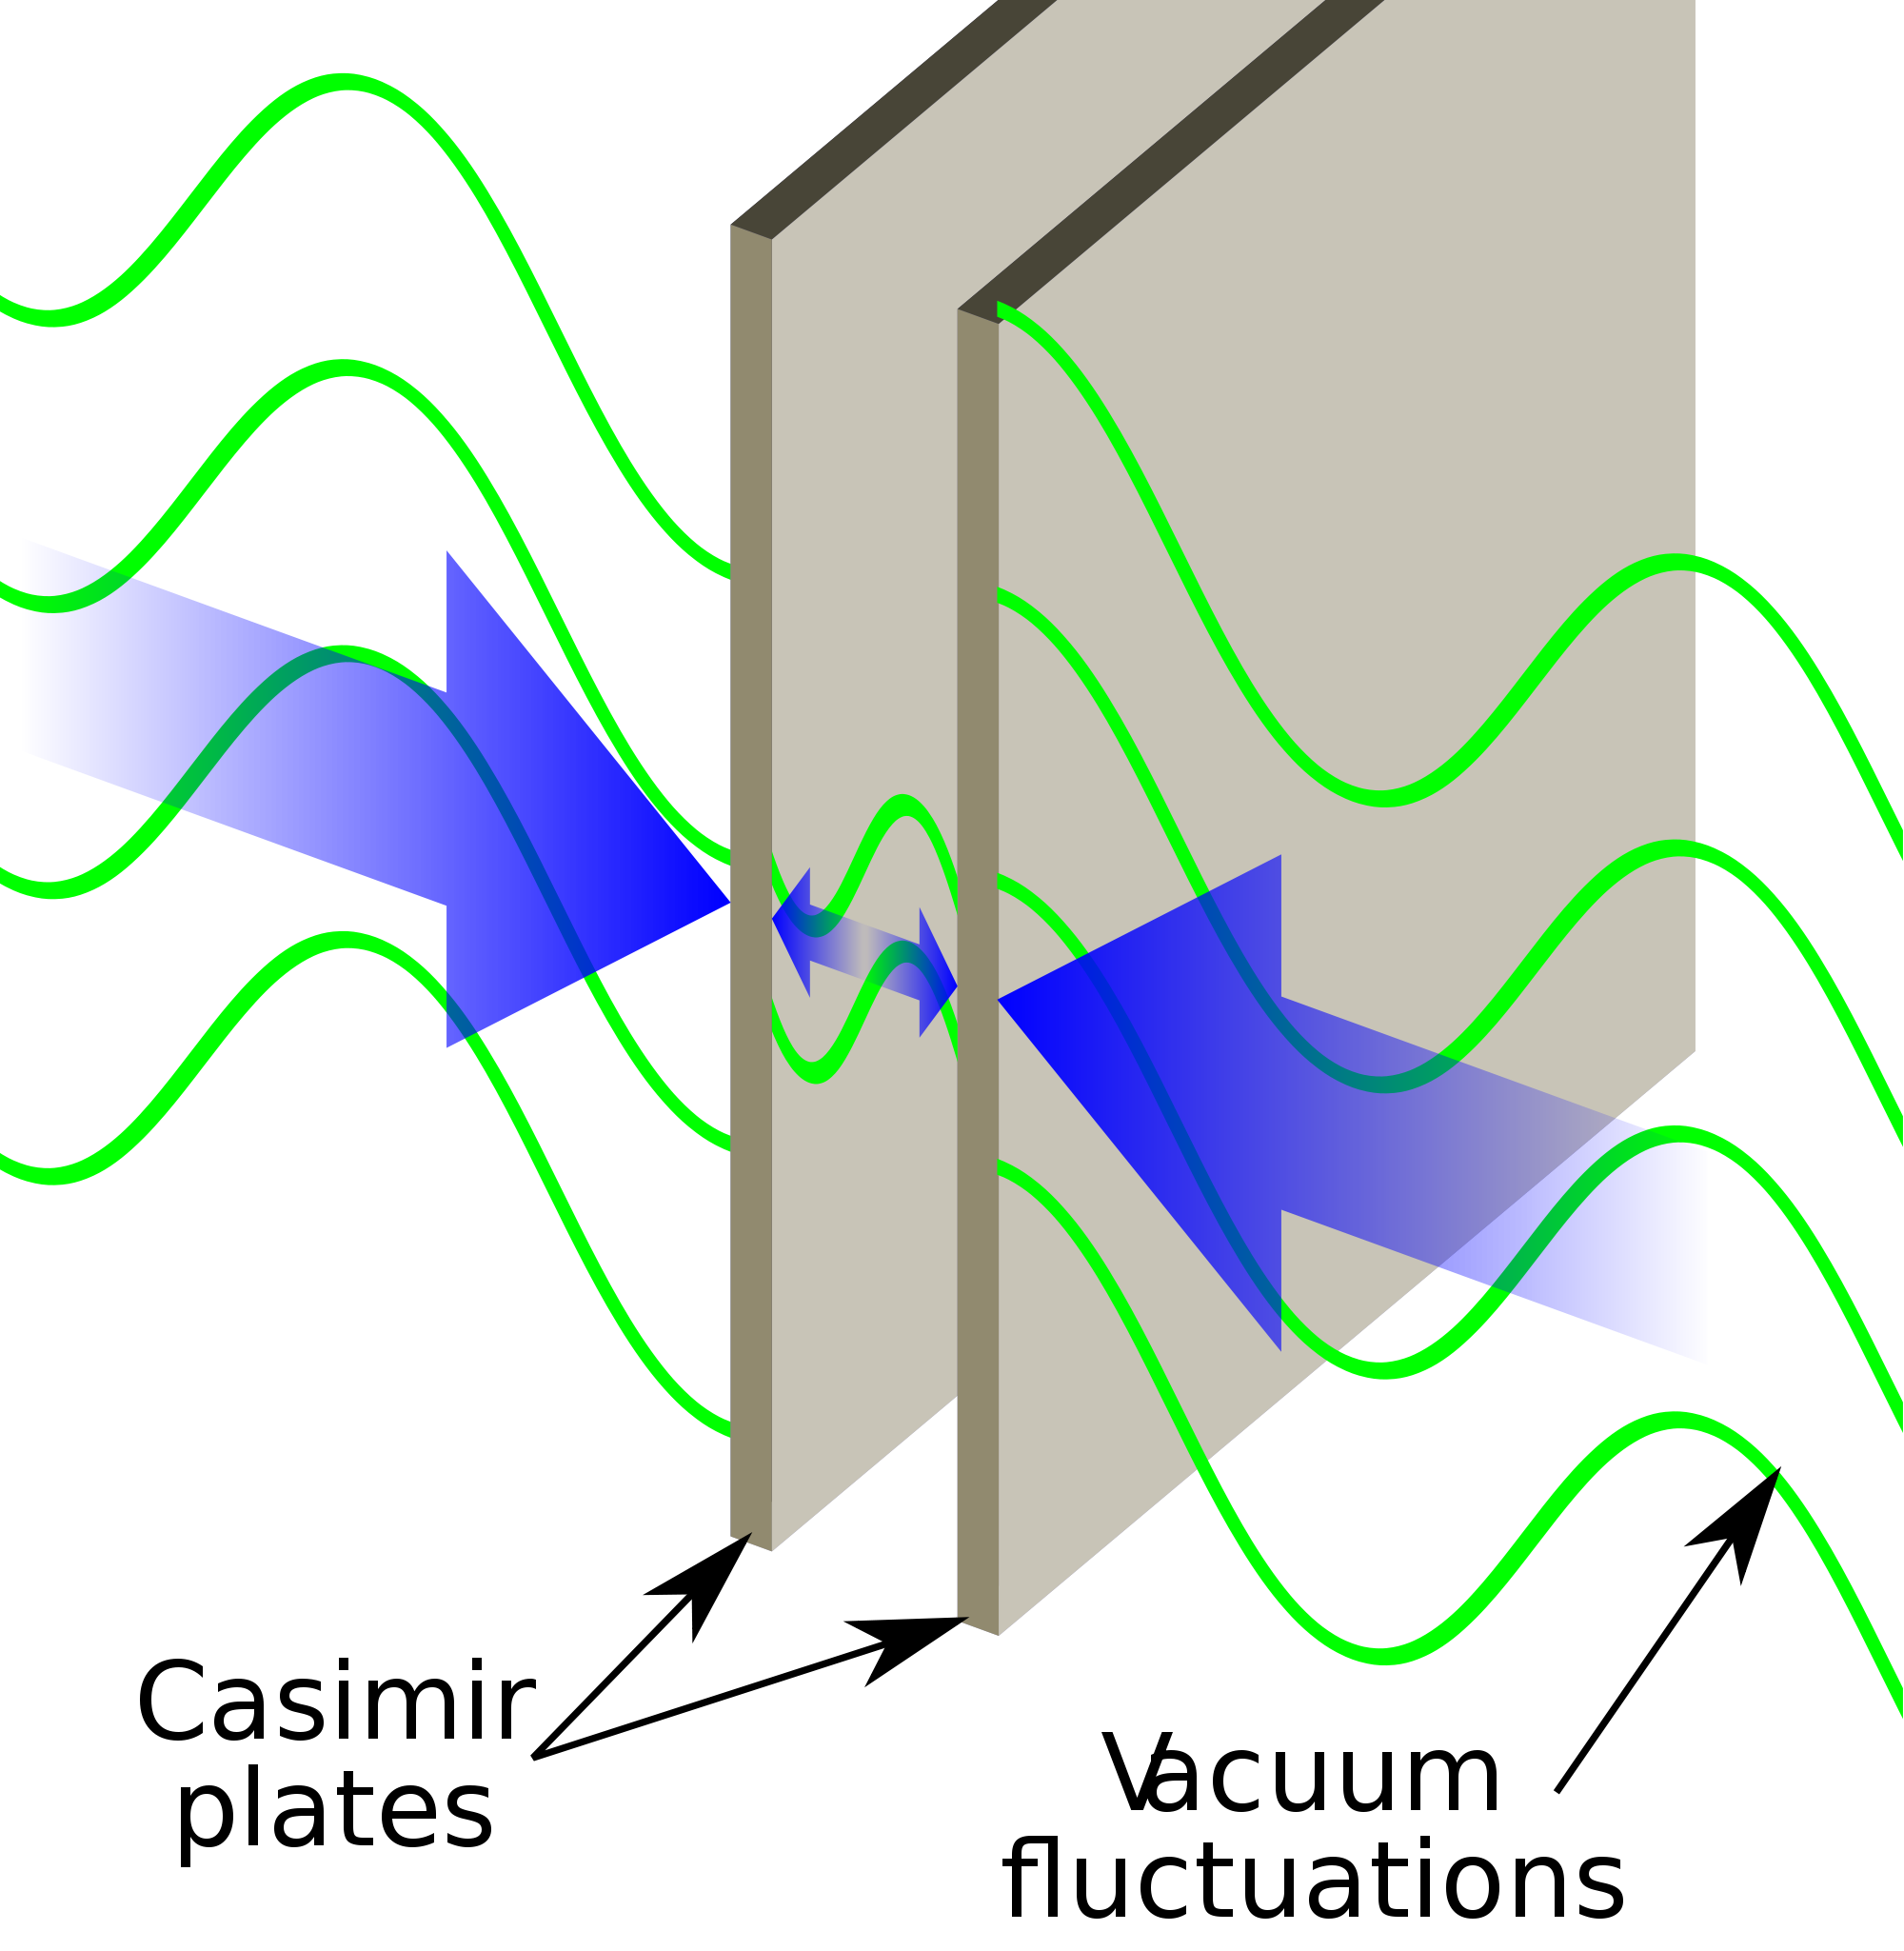
\includegraphics[width=0.6\linewidth]{plates}
		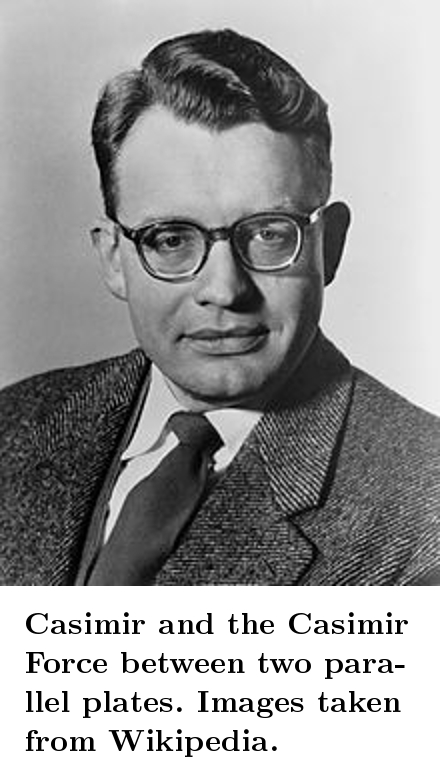
\includegraphics[width=0.35\linewidth]{casimir3}
	\end{center}
The Casimir effect extends quantum field theory to allow for negative energy densities. It has been suggested by numerous physicists such as Stephen Hawking, Kip Thorne, and others that such a thing will allow the possibilities of stabilizing traversable wormholes. Miguel Alcubierre, creator of the Alcubierre Drive has also suggested using the Casimir effect to obtain the negative energy required for his designs. Other possible applications include propulsion drives for space craft and nano-technology.
\end{multicols}
}

%----------------------------------------------------------------------------------------
%	Astounding Mathematics
%----------------------------------------------------------------------------------------

\headerbox{Computational Models}{name=method,column=3,below=objectives,bottomaligned=conclusion}{ % This block's bottom aligns with the bottom of the conclusion block
\small{
	
	
	
%Consider the following well defined sum ($x<1$) 
%\begin{align}
%&f(x) = 1+x+x^2+x^3+\cdots = (1-x)^{-1} \\
%&\implies f'(x)=1+2x+3x^2+\cdots = (1-x)^{-2}.
%\end{align}
%If we evaluate this at $x=-1$ we get
%\begin{align}
%f'(-1) = 1-2+3-4+\cdots = 1/4.
%\end{align}
%Now, if we take $2^{-s} \zeta(s)$ we have
%\begin{align}
%2^{-s} \zeta(s)  = 2^{-s} + 4^{-s}+6^{-s}+8^{-s}\cdots.
%\end{align}
%Now, if we take $g(s)=[1-2(2^{-s})]\zeta(s)$ we have
%\begin{align}
%g(s) &= 1-2^{-s}+3^{-s}-4^{-s}+5^{-s}-\cdots.
%\end{align}
%If we set $s=-1$, we can see that $g(-1)= -3\zeta(-1)$ and so
%\begin{align}
%-3\zeta(-1) &= 1-2+3-4+\cdots = 1/4  \\
%&\implies \zeta(-1) = -1/12.
%\end{align}
%Now, notice that plugging in $s=-1$ into the Riemann zeta function gives
%\begin{align}
%\zeta(-1) = -\frac{1}{12} \implies \sum_{n=1}^{\infty}n \rightarrow -\frac{1}{12}.
%\end{align}
}}

%----------------------------------------------------------------------------------------
%	Analytic Continuation
%----------------------------------------------------------------------------------------

\headerbox{Land\'{e}  g Factor}{name=results2,column=0,below=objectives,bottomaligned=conclusion}{ % This block's bottom aligns with the bottom of the conclusion block
\small{
In quantum physics, the energy density should be $S(-3) = 1+8+27+64+\cdots$, which is a divergent series and thus does not make much sense as an energy density. When we use the process of analytic continuation, this can be written as
\begin{align}
\zeta(-3) = 1+2^3+3^3+4^3 +\cdots \rightarrow 1/120 \label{eq:ZetaNeg3}.
\end{align}
The way Ramanujin expresses functions that are divergent such as this [\ref{ramanujin}] (from the Riemann zeta function) is
\small{\begin{align}
\sum_{k=\alpha}^{x} f(k) \sim \int_{\alpha}^{x}f(t) dt+c+\frac{1}{2}f(x) \nonumber \\+\sum_{k=1}^{\infty}\frac{B_{2k}}{(2k)!}f^{(2k-1)}(x).
\end{align}}This is a process of analytically continuing these divergent series and coming up with a finite result without any 'magic'. I say magic because there is a process, which was first shown by Euler around 1735 [\ref{baez}], in which one can ignore the divergent nature of a sum and come up with these results as well. An example is demonstrated in the right panel which is a result that is very important to obtaining the $24+2=26$ dimensions in bosonic string theory. It is also a simpler example than that of equation (\ref{eq:ZetaNeg3}) to demonstrate.
}}

%----------------------------------------------------------------------------------------

\end{poster}

\end{document}